\documentclass{beamer}
\usepackage{amsmath}
\usepackage{rotating}
\usepackage{graphicx}
\usepackage{multimedia}


\useinnertheme[shadow=true]{rounded}
\useoutertheme{shadow}
\usecolortheme{orchid}
\usecolortheme{whale}

\mode<presentation>

\newcommand{\dif}{\, \mathrm{d}}
\newcommand{\diff}[2]{\frac{\mathrm{d}#1}{\mathrm{d}#2}}
\newcommand{\partdiff}[2]{\frac{\partial #1}{\partial #2}}


\title{TMA4280 - Introduction to supercomputing}
\subtitle{Message passing and MPI}
\author{Einar M. R{\o}nquist}
\institute{NTNU}
\date{January 2011}

\begin{document}

\maketitle

\begin{frame}\frametitle{The message-passing model}
\begin{center}
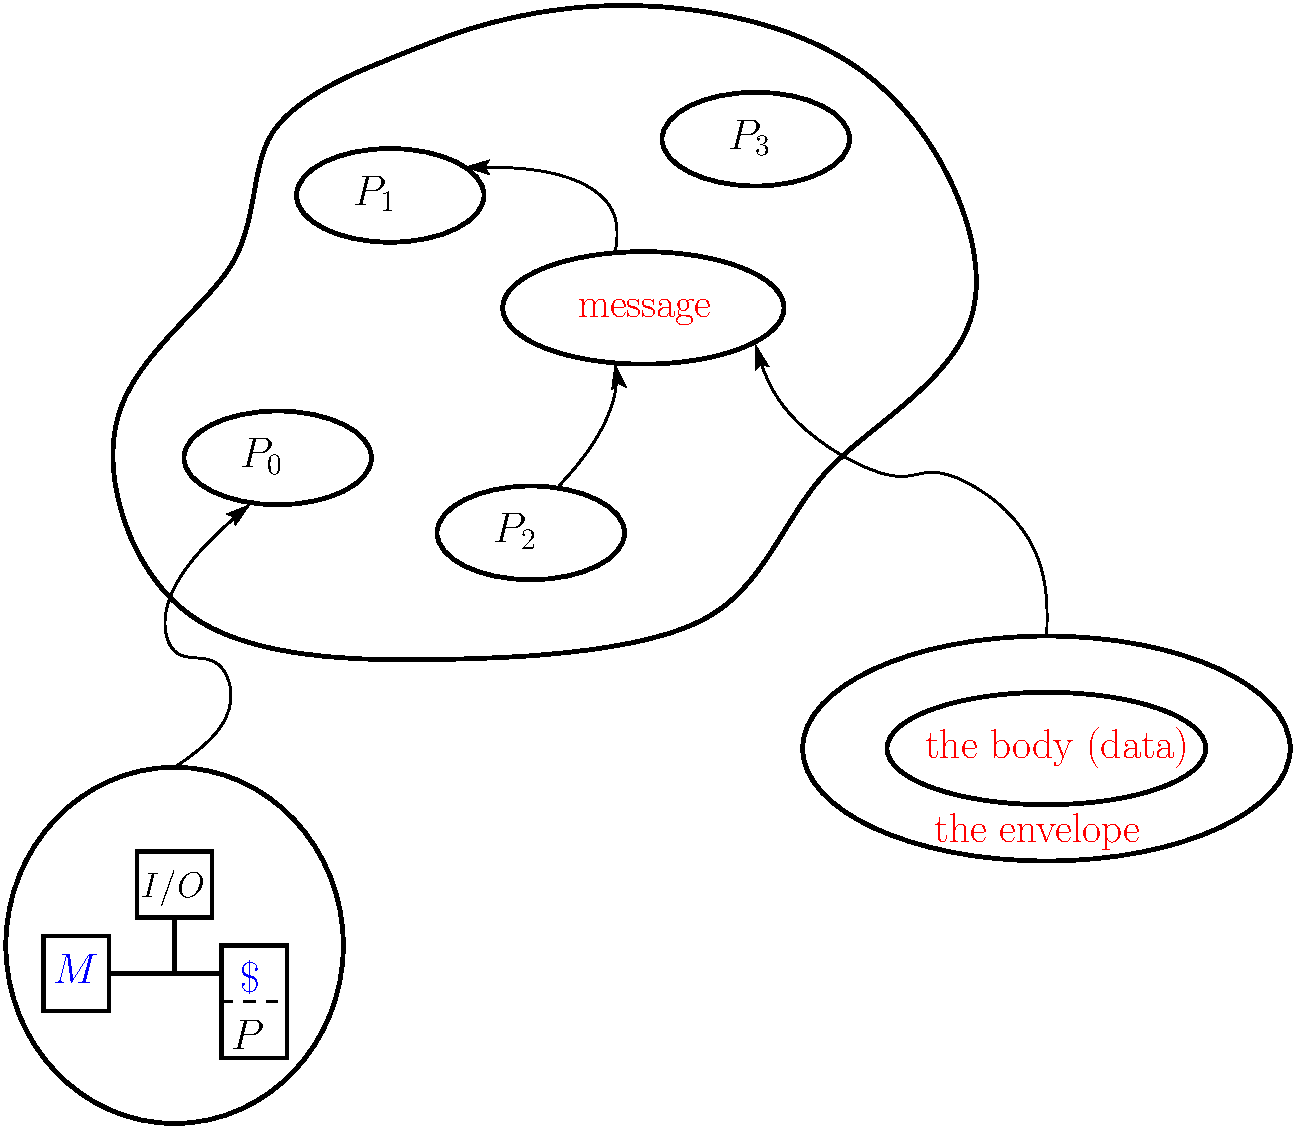
\includegraphics[width=9cm]{message_passing_model}
\end{center}
\end{frame}

\begin{frame}\frametitle{An example using MPI together with C}

\texttt{\#include <stdio.h> }\\
\texttt{\#include <mpi.h>}\\
\vspace{.1in}
\texttt{int main(int argc, char **argv)}\\
\texttt{\{}\\
\texttt{ \hspace{0.5cm}     int rank, size, tag, i; } \\
\texttt{ \hspace{0.5cm}     \textcolor{red}{MPI\_Status} status;}\\
\texttt{ \hspace{0.5cm}     char message[20]; }\\
\vspace{.1in}
\texttt{ \hspace{0.5cm}     \textcolor{red}{MPI\_Init} (\&argc, \&argv);}\\
\texttt{ \hspace{0.5cm}      \textcolor{red}{MPI\_Comm\_size} 
(MPI\_COMM\_WORLD, \&size);}\\
\texttt{ \hspace{0.5cm}      \textcolor{red}{MPI\_Comm\_rank} 
(MPI\_COMM\_WORLD, \&rank);}\\
\vspace{.1in}
\texttt{ \hspace{0.5cm}     tag = 100;}\\
\vspace{.1in}
%\texttt{ \hspace{0.5cm}     if (rank == 0) \{ }\\

\end{frame}


\begin{frame}\frametitle{An example using MPI together with C}

\texttt{ \hspace{0.5cm}     if (rank == 0) \{ }\\
\texttt{ \hspace{1cm}     strcpy (message, "Hello, world"); }\\
\texttt{ \hspace{1cm}     for (i=1; i < size; i++) \{ }\\
\texttt{ \hspace{1.5cm}      \textcolor{red}{MPI\_Send} (message, 13, MPI\_CHAR, i, tag, }\\
\texttt{ \hspace{6.5cm}  MPI\_COMM\_WORLD);}\\
\texttt{ \hspace{1cm} \} }\\
\texttt{ \hspace{0.5cm}     \} }\\
\texttt{ \hspace{0.5cm}   else \{ }\\
\texttt{ \hspace{1cm}    \textcolor{red}{MPI\_Recv} (message, 13, MPI\_CHAR, 0, tag, }\\
\texttt{ \hspace{4.5cm} MPI\_COMM\_WORLD, \&status); }\\
\texttt{ \hspace{0.5cm}     \} }\\
\vspace{.1in}
\texttt{ \hspace{0.5cm}  printf ( "process \%d :  \%s $\backslash$n", rank, message); }\\
\vspace{.1in}
\texttt{ \hspace{0.5cm}  \textcolor{red}{MPI\_Finalize}(); }\\
\vspace{.1in}
\texttt{ \hspace{0.5cm} return(0);}\\
\texttt{\}}\\
\end{frame}

\begin{frame}\frametitle{An example using MPI together with FORTRAN}

\texttt{ \hspace{0.5cm}  program hello} \\
\texttt{ \hspace{0.5cm}  include 'mpif.h' } \\
\vspace{.1in}
\texttt{ \hspace{0.5cm}  integer rank, size, ierror, tag }\\
\texttt{ \hspace{0.5cm}  integer status(MPI\_STATUS\_SIZE)}\\
\texttt{ \hspace{0.5cm}  character(12) message }\\
\vspace{.2in}
\texttt{ \hspace{0.5cm}  \textcolor{red}{call MPI\_INIT} (ierror);} \\
\texttt{ \hspace{0.5cm}  \textcolor{red}{call MPI\_COMM\_SIZE} 
(MPI\_COMM\_WORLD, size, ierror);}\\
\texttt{ \hspace{0.5cm}  \textcolor{red}{call MPI\_COMM\_RANK} 
(MPI\_COMM\_WORLD, rank, ierror);}\\
\vspace{.2in}
\texttt{ \hspace{0.5cm}  tag = 100; }\\
\end{frame}

\begin{frame}\frametitle{An example using MPI together with FORTRAN}
\texttt{ \hspace{0.5cm}  if (rank .eq. 0) then}\\ 
\texttt{ \hspace{1cm} message = 'Hello, world'}\\
\texttt{ \hspace{1cm}  do i=1, size-1}\\
\texttt{ \hspace{1.5cm}    \textcolor{red}{call MPI\_SEND} (message, 12, MPI\_CHARACTER, }\\ 
\texttt{ \hspace{0.45cm}\$         \hspace{3cm}        i, tag, MPI\_COMM\_WORLD, ierror)}\\
\texttt{ \hspace{1cm}     enddo}\\
\texttt{ \hspace{0.5cm} else}\\
\texttt{ \hspace{1.5cm}   \textcolor{red}{call MPI\_RECV} (message, 12, MPI\_CHARACTER, }\\
\texttt{ \hspace{0.45cm}\$       \hspace{1.5cm}        0, tag, MPI\_COMM\_WORLD, status, ierror)}\\
\texttt{ \hspace{0.5cm} endif}\\
\vspace{.1in}   
\texttt{ \hspace{0.5cm} print*, 'process', rank, ':' message}\\
 \vspace{.1in}        
\texttt{ \hspace{0.5cm} \textcolor{red}{call MPI\_Finalize} (ierror)}\\
\vspace{.1in}
\texttt{ \hspace{0.5cm} end}
\end{frame}

\begin{frame}\frametitle{An example using MPI: output using $P=4$ processors}

\texttt{  node 0 :   Hello, world}\\
\texttt{  node 1 :   Hello, world}\\
\texttt{  node 3 :   Hello, world}\\
\texttt{  node 2 :   Hello, world}
\end{frame}

\begin{frame}\frametitle{MPI - Message Passing Interface}
Advantages of the MPI message-passing model:
\vspace{.1in}
\begin{itemize}
\item standardization; 
\item portability;
\item performance; 
\item expressiveness. 
\end{itemize}
\vspace{.2in}
MPI is a library comprising about 125 functions or operations: 
\vspace{.1in}
\begin{itemize}
\item \textcolor{red}{one-to-one} operations (or point-to-point communication); 
\item \textcolor{red}{one-to-all} operations; 
\item \textcolor{red}{all-to-one} operations; 
\item \textcolor{red}{all-to-all} operations. 
\end{itemize}
\vspace{.2in}
The last three types are referred to as {\em collective} operations. 
\end{frame}

\begin{frame}\frametitle{MPI: header file}
Header file required: \\
\vspace{.4in}
\texttt{C: \hspace{2cm} \#include "mpi.h"}\\
\vspace{.2in}
\texttt{FORTRAN: \hspace{1cm} include 'mpif.h'}
\end{frame}


\begin{frame}\frametitle{MPI: format}

\texttt{C: \hspace{2cm} \textcolor{blue}{ec} = \textcolor{red}{MPI\_Xxxxx} (parameters,...); }\\
\vspace{.2in}
or simply\\
\vspace{.2in}
\texttt{C: \hspace{3cm} \textcolor{red}{MPI\_Xxxxx} (parameters,...); }\\
\vspace{.5in}
\texttt{FORTRAN: \hspace{0.9cm} 
\textcolor{red}{call MPI\_XXXXX} (parameters,...,\textcolor{blue}{ierr}) }
\end{frame}

\begin{frame}\frametitle{MPI: six essential functions}
\begin{tabular}{ll}
\textcolor{blue}{C} & \hspace{3cm}\textcolor{blue}{FORTRAN} \\
\vspace{.1in} & \vspace{.1in}\\
\texttt{MPI\_Init} &  \hspace{3cm}\texttt{call MPI\_INIT}  \\
\texttt{MPI\_Comm\_size} & \hspace{3cm}\texttt{call MPI\_COMM\_SIZE} \\
\texttt{MPI\_Comm\_rank}  &  \hspace{3cm}\texttt{call MPI\_COMM\_RANK}\\
\texttt{MPI\_Send}  & \hspace{3cm}\texttt{call MPI\_SEND}  \\
\texttt{MPI\_Recv}  & \hspace{3cm}\texttt{call MPI\_RECV}\\
\texttt{MPI\_Finalize} & \hspace{3cm}\texttt{call MPI\_FINALIZE}
\end{tabular}
\end{frame}

\begin{frame}\frametitle{MPI: \hspace{1cm}message = data + envelope}
\texttt{\textcolor{red}{MPI\_Send} ($\underbrace{buffer, count, datatype}_{\textcolor{blue}{data}}$, 
$\underbrace{dest, tag, comm}_{\textcolor{blue}{envelope}}$); } \\
\vspace{.4in}
\texttt{\textcolor{red}{MPI\_Recv} ($\underbrace{buffer, count, datatype}_{\textcolor{blue}{data}}$, 
$\underbrace{source, tag, comm,\&status}_{\textcolor{blue}{envelope}}$); } \\
\vspace{.5in}
Examples of predefined data types (C): \\
\vspace{.2in}
\texttt{MPI\_CHAR}\\
\texttt{MPI\_INT}\\
\texttt{MPI\_FLOAT}\\
\texttt{MPI\_DOUBLE}
\end{frame}

\begin{frame}\frametitle{MPI: point-to-point communication}
\texttt{\textcolor{red}{MPI\_Send}}�
and \texttt{\textcolor{red}{MPI\_Recv}}: \textcolor{blue}{blocking} send and receive\\
\vspace{.4in}
\begin{tabular}{ll}
Deadlock example:  & \hspace{1.5cm}Solution: \\
\vspace{.1in} & \vspace{.1in} \\
\texttt{if (rank == 0) \{ }     &  
\hspace{1.5cm}\texttt{if (rank == 0) \{ }\\
\texttt{\hspace{.5cm}\textcolor{red}{MPI\_Recv} (...); }  & 
\hspace{1.5cm}\texttt{\hspace{.5cm}\textcolor{red}{MPI\_Send} (...); } \\
\texttt{\hspace{.5cm}\textcolor{red}{MPI\_Send} (...); }  & 
\hspace{1.5cm}\texttt{\hspace{.5cm}\textcolor{red}{MPI\_Recv} (...); } \\
\texttt{\}}  & \hspace{1.5cm}\texttt{\}}   \\
\texttt{elseif (rank == 1) \{ }  & \hspace{1.5cm}\texttt{elseif (rank == 1) \{ } \\
\texttt{\hspace{.5cm}\textcolor{red}{MPI\_Recv} (...); }  & 
\hspace{1.5cm}\texttt{\hspace{.5cm}\textcolor{red}{MPI\_Recv} (...); } \\
\texttt{\hspace{.5cm}\textcolor{red}{MPI\_Send} (...); } &
\hspace{1.5cm}\texttt{\hspace{.5cm}\textcolor{red}{MPI\_Send} (...); }  \\
\texttt{\}} & \hspace{1.5cm}\texttt{\}} 
\end{tabular}

\end{frame}

\begin{frame}\frametitle{MPI: collective operations}
In general: \\
\begin{itemize}
\item involve all of the processes in a group; 
\item more efficient and less tedious to use compared to point-to-point communication. 
\end{itemize}
\vspace{.5in}
Example (syncronization): \\
\vspace{.2in}
\texttt{\textcolor{red}{MPI\_Barrier} (comm);} 
\end{frame}

\begin{frame}\frametitle{MPI: collective operations (ref: Foster)}
\begin{center}
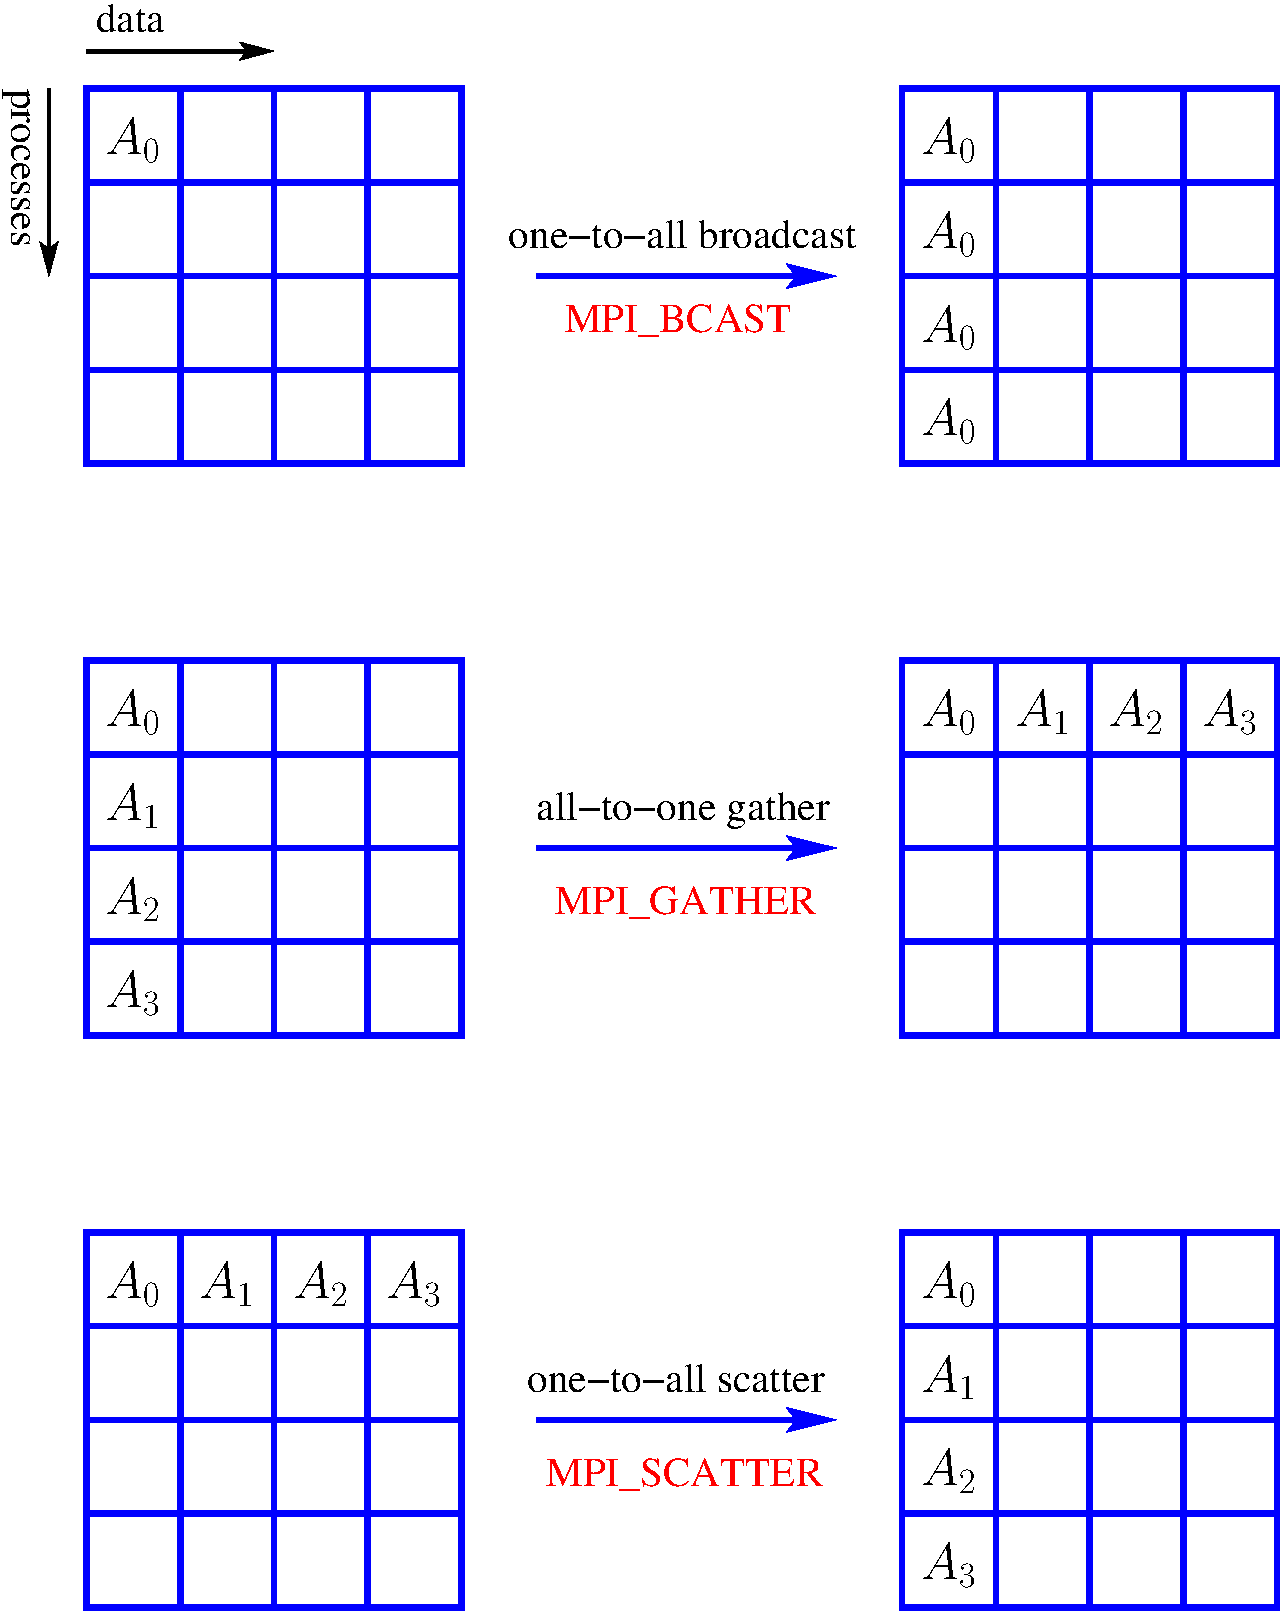
\includegraphics[width=9cm]{mpi_op1}
\end{center}
\end{frame}

\begin{frame}\frametitle{MPI: global reduction or combine operations (ref: Foster)}
\begin{center}
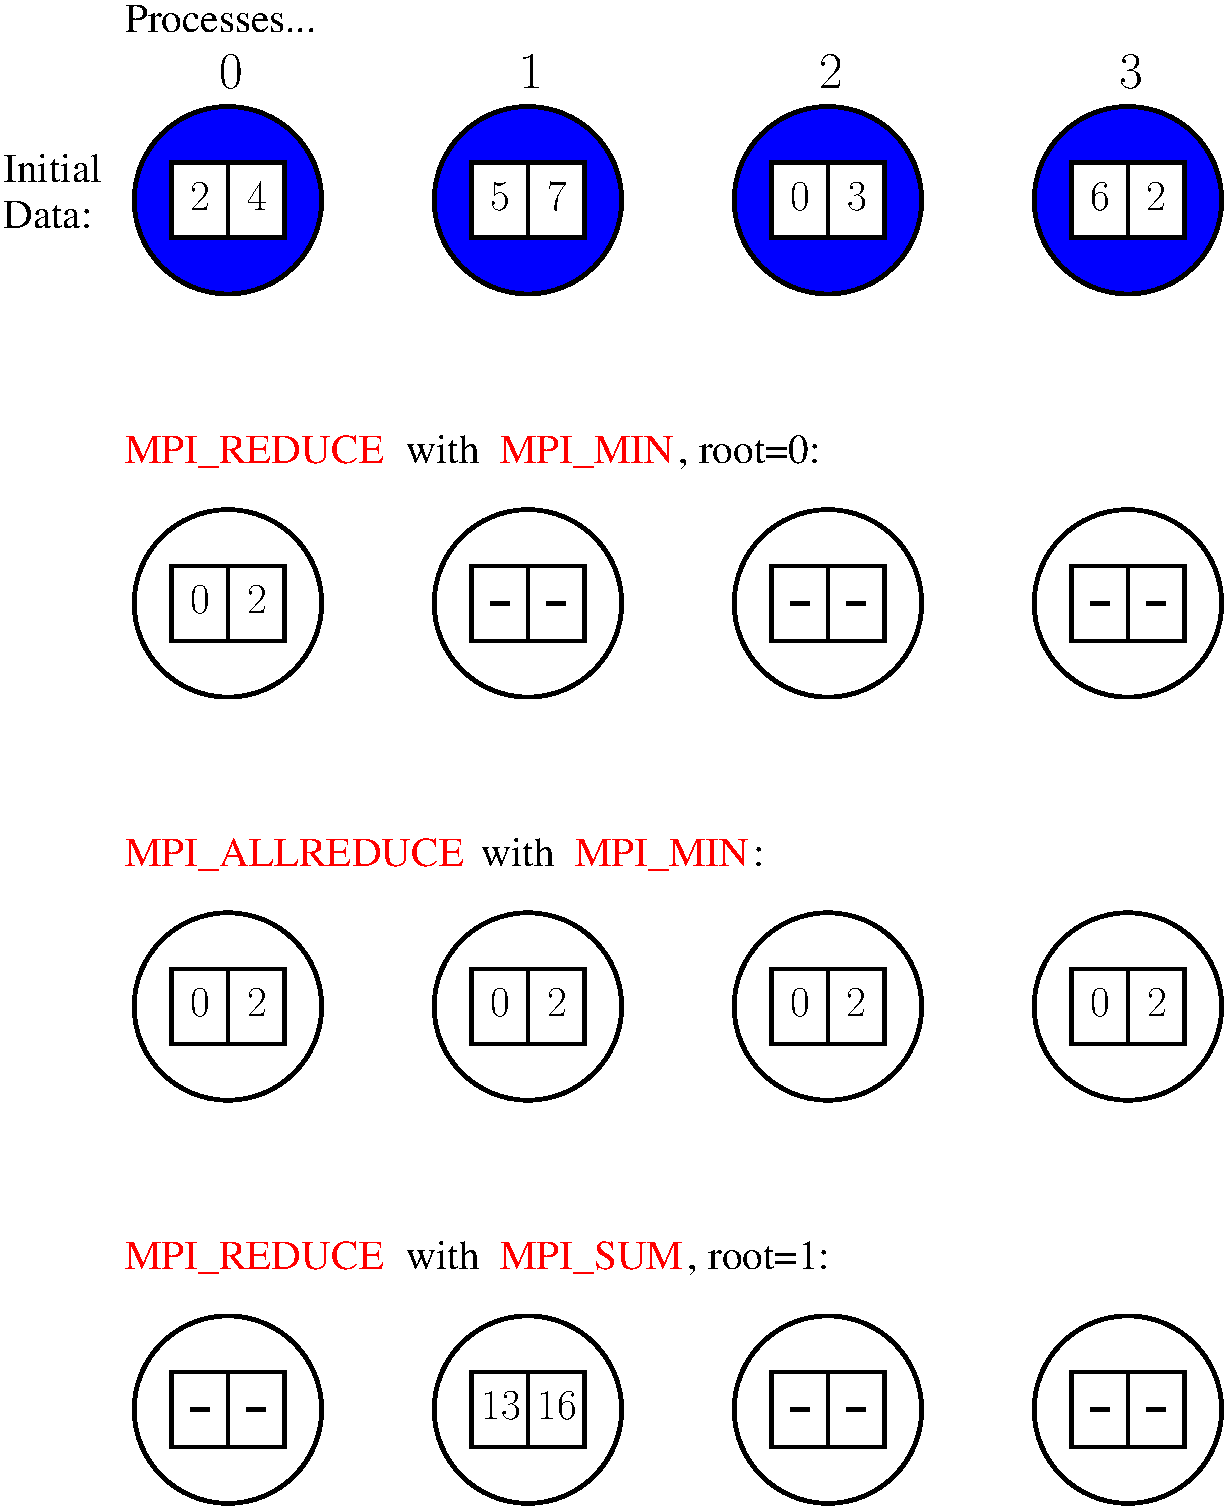
\includegraphics[width=9cm]{mpi_op2}
\end{center}
\end{frame}

\begin{frame}\frametitle{MPI: global reduction operations}

\texttt{\textcolor{red}{MPI\_Reduce} ($\underbrace{sbuf, rbuf,count, datatype}_{\textcolor{blue}{data}}$, 
$\underbrace{op, root, comm}_{\textcolor{blue}{envelope}}$); } \\
\vspace{.4in}
\texttt{\textcolor{red}{MPI\_Allreduce} ($\underbrace{sbuf, rbuf,count, datatype}_{\textcolor{blue}{data}}$, 
$\underbrace{op, comm}_{\textcolor{blue}{envelope}}$); } \\
\vspace{.4in}
Examples of predefined operations (C): \\
\vspace{.2in}
\texttt{MPI\_SUM}\\
\texttt{MPI\_PROD}\\
\texttt{MPI\_MIN}\\
\texttt{MPI\_MAX}
\end{frame}

\begin{frame}\frametitle{A ``problem'': defining $\pi$ through integration}
\begin{align*}
\int_0^1\frac{1}{1+x^2} \dif{x} &= [\textrm{arctan}(x)]_0^1 \\
 &= \textrm{arctan}(1) - \textrm{arctan}(0) 
 = \frac{\pi}{4}
\end{align*}
Hence,
\begin{align*}
\pi = \int_0^1\frac{4}{1+x^2} \dif{x}
\end{align*}
\end{frame}

\begin{frame}\frametitle{Numerical integration  ($h=1/n$)}
\begin{center}
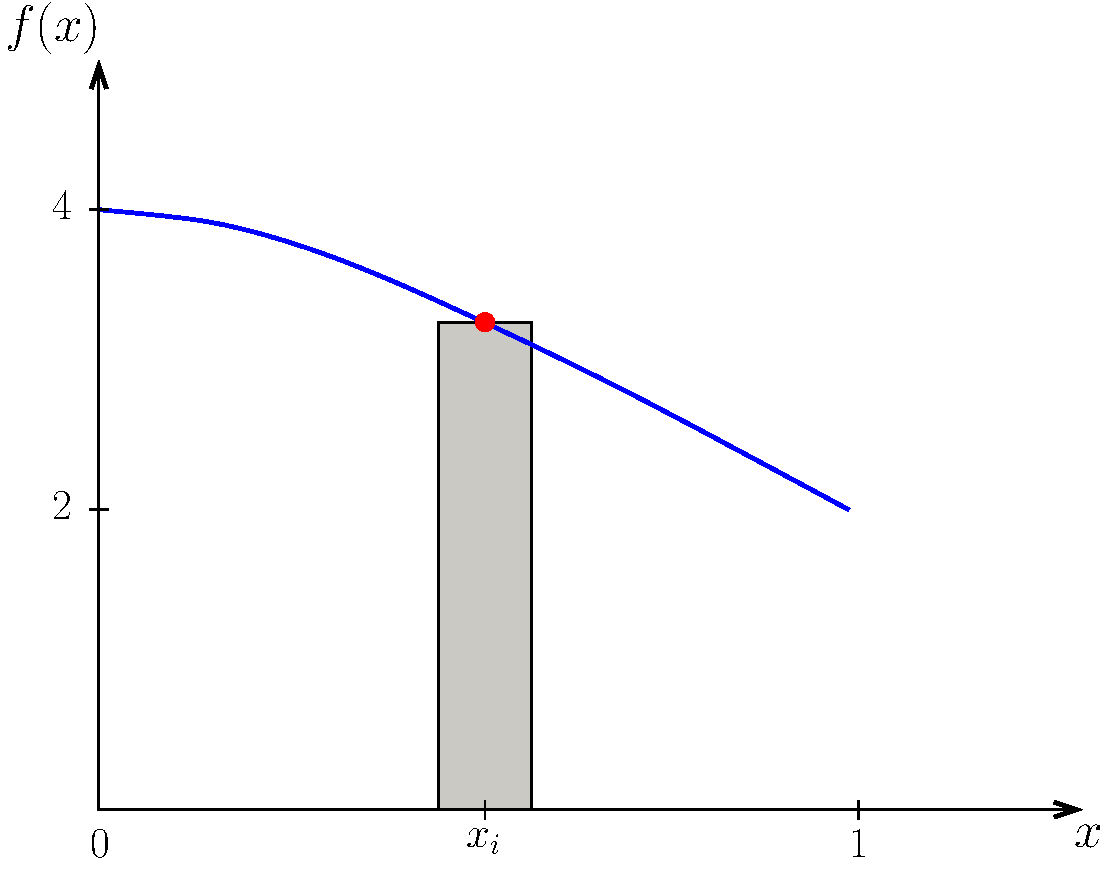
\includegraphics[width=6cm]{Midpoint}
\end{center}
The grey area:  
\begin{align*}
\left ( \frac{4}{1+x_i^2} \right ) \cdot h, \qquad \text{with}\quad x_i = \left (i-\frac{1}{2} \right )\cdot h
\end{align*}
and 
\begin{align*}
i=1,\ldots,n
\end{align*}
\end{frame}

\begin{frame}\frametitle{Numerical integration}
Exact value: 
\begin{align*}
\pi = \int_0^1\frac{4}{1+x^2} \dif{x}
\end{align*}
\vspace{.5in}

Approximation (midpoint rule):

\begin{align*}
\pi_n = \sum_{i=1}^n \left (\frac{4}{1+x_i^2} \right ) \cdot h
\end{align*}
\end{frame}

\begin{frame}\frametitle{Parallel programming using MPI together with C}
\texttt{\#include <stdlib.h> }\\
\texttt{\#include <stdio.h> }\\
\texttt{\#include <math.h> }\\
\texttt{\#include <mpi.h>}\\
\vspace{.1in}
\texttt{int main(int argc, char **argv)}\\
\texttt{\{}\\
\texttt{ \hspace{0.5cm}     double mypi, pi, h, sum, x, piref, error; } \\
\texttt{ \hspace{0.5cm}     double t1, t2, dt; } \\
\texttt{ \hspace{0.5cm}     int n, myid, nproc, i; } \\
\vspace{.1in}
\texttt{ \hspace{0.5cm}     \textcolor{red}{MPI\_Init} (\&argc, \&argv);}\\
\texttt{ \hspace{0.5cm}      \textcolor{red}{MPI\_Comm\_size} 
(MPI\_COMM\_WORLD, \&nproc);}\\
\texttt{ \hspace{0.5cm}      \textcolor{red}{MPI\_Comm\_rank} 
(MPI\_COMM\_WORLD, \&myid);}\\
\vspace{.1in}
\end{frame}

\begin{frame}\frametitle{An example using MPI together with C}
\texttt{ \hspace{0.5cm}     if (myid == 0) \{ }\\
\texttt{ \hspace{1cm}     printf (" Enter the number of intervals:$\backslash$n"); }\\
\texttt{ \hspace{1cm}     scanf ("\%d",\&n); }\\
\texttt{ \hspace{1cm}      t1 = \textcolor{red}{MPI\_Wtime()}; }\\
\texttt{ \hspace{0.5cm}     \} }\\
\texttt{ \hspace{0.5cm}    \textcolor{red}{ MPI\_Bcast} (\&n, 1, MPI\_INT, 0, MPI\_COMM\_WORLD);}\\
\vspace{.1in}
\texttt{ \hspace{0.5cm}  if (n > 0) \{  }\\
\texttt{ \hspace{1cm}   h = 1.0 / (double)n;  }\\
\texttt{ \hspace{1cm}   sum = 0.0;  }\\
\texttt{ \hspace{1cm}    for (i = myid+1; i <= n; i += nproc) \{  }\\
\texttt{ \hspace{1.5cm}  x = h * ((double)i - 0.5);  }\\
\texttt{ \hspace{1.5cm}   sum = sum + (4.0 / (1.0 + x*x)); }\\
\texttt{ \hspace{1cm}     \} }\\
\texttt{ \hspace{1cm}    mypi = h * sum; }\\
\vspace{.1in}
\texttt{ \hspace{1cm}  MPI\_Reduce (\&mypi, \&pi, 1, MPI\_DOUBLE, MPI\_SUM, }\\
\texttt{ \hspace{6.5cm}     0, MPI\_COMM\_WORLD);  }
\end{frame}

\begin{frame}\frametitle{An example using MPI together with C}
\texttt{ \hspace{1cm}  if (myid ==  0) \{  }\\
\texttt{ \hspace{1.5cm}  t2 = \textcolor{red}{MPI\_Wtime()};  }\\
\texttt{ \hspace{1.5cm}  dt = t2 - t1; }\\
\texttt{ \hspace{1.5cm} piref = 4.0 * atan(1.0); }\\
\texttt{ \hspace{1.5cm} error = fabs(pi-piref); }\\
\texttt{ \hspace{1.5cm} printf (" pi= \%e  error= \%e  dt= \%e $\backslash$n", }\\
\texttt{ \hspace{6.5cm}pi, error, dt);}\\
\texttt{ \hspace{1cm}     \} }\\
\texttt{ \hspace{0.5cm}     \} }\\
\vspace{.1in}
\texttt{ \hspace{0.5cm}  \textcolor{red}{MPI\_Finalize}(); }\\
\vspace{.1in}
\texttt{ \hspace{0.5cm} return(0);}\\
\texttt{\}}\\
\end{frame}

\begin{frame}\frametitle{Questions}
\begin{enumerate}
\item Is the program correct, \\e.g., is the convergence rate as expected?
\vspace{.1in}
\item Is the program load-balanced?
\vspace{.1in}
\item Do we get the same value of $\pi_n$ for different values of $P$?
\vspace{.1in}
\item Is the program scalable?
\end{enumerate}
\end{frame}

\begin{frame}\frametitle{Correctness: convergence test}
\begin{center}
\begin{tabular}{|c|c|c|c|c|c|c|c|} \hline
$n$ & $\textrm{error} = |\pi - \pi_n |$
  \\ \hline
10 & $8.33\cdot 10^{-4}$
  \\ \hline
$10^2$ & $8.33\cdot 10^{-6}$
  \\ \hline
$10^3$ & $8.33\cdot 10^{-8}$
  \\ \hline
$10^4$ & $8.33\cdot 10^{-10}$
  \\ \hline
$10^5$ & $8.37\cdot 10^{-12}$
  \\ \hline
\end{tabular}
\end{center}
Hence, 
\begin{align*}
|\pi - \pi_n | \sim {\cal O}(h^2)
\end{align*}
where 
\begin{align*}
h = 1/n
\end{align*}
\end{frame}

\begin{frame}\frametitle{Scalability: timing results on \texttt{gridur}}
\begin{center}
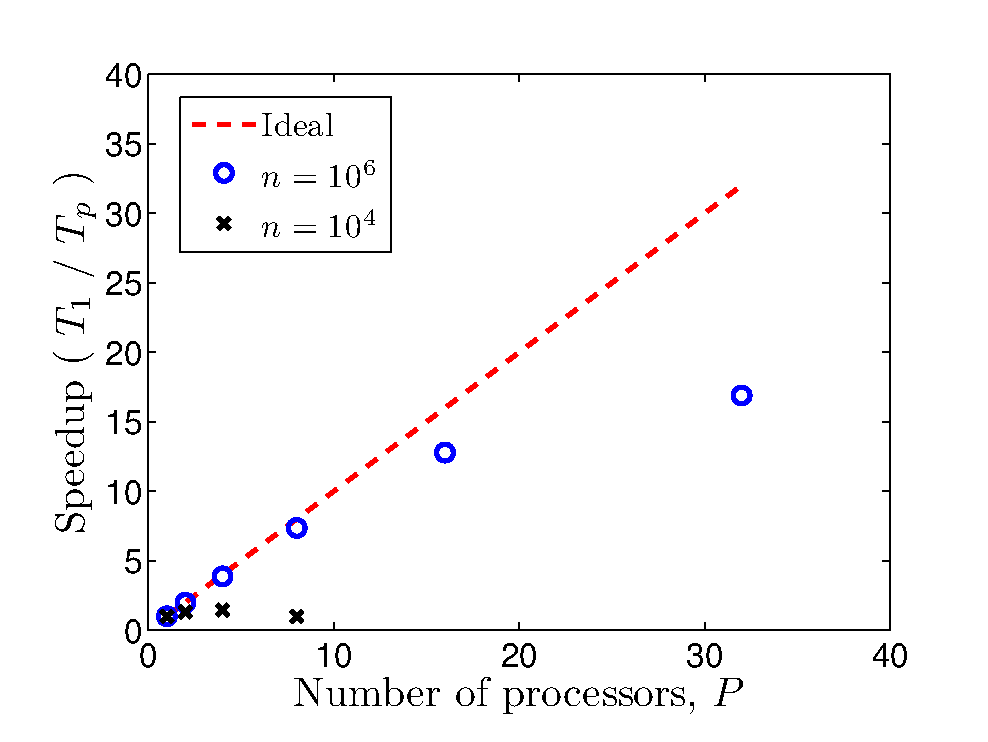
\includegraphics[width=10cm]{pi_sp_new}
\end{center}
\end{frame}

\begin{frame}\frametitle{The innerproduct }
\begin{align*}
\sigma = \underline{x}^T\underline{y} = \underline{x}\cdot\underline{y}
\end{align*}
\begin{align*}
\sigma = \sum_{m=0}^{M-1} x_m y_m
\end{align*}

\vspace{0.5cm}

\begin{center}
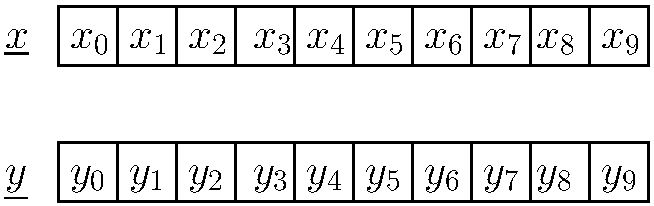
\includegraphics[width=8cm]{Vector1}
\end{center}
\end{frame}


\begin{frame}\frametitle{The innerproduct: distribution of work }
\begin{center}
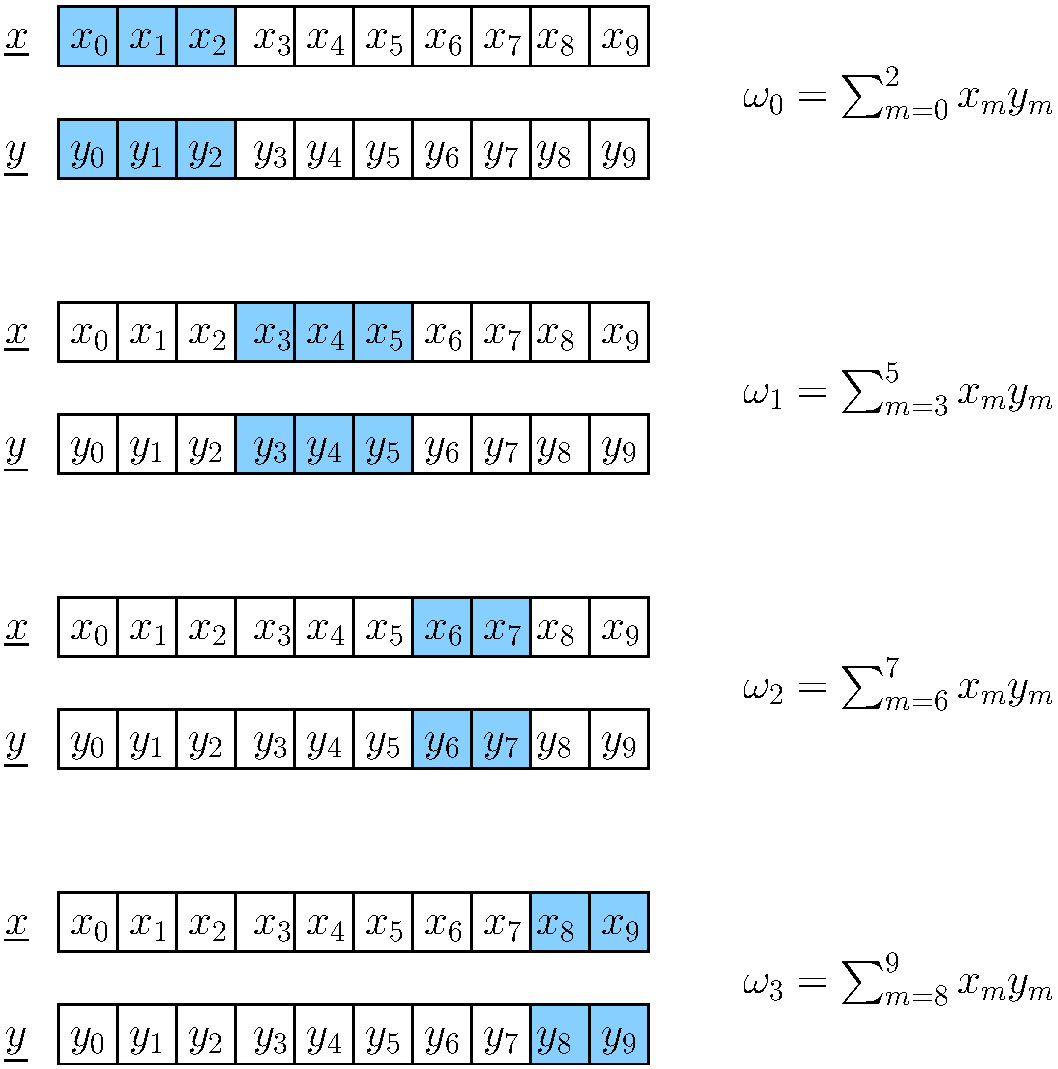
\includegraphics[width=7.5cm]{Vector2}
\end{center}
\end{frame}


\begin{frame}\frametitle{Sample "program" on processor $p$, ($0 \leq p < P$)}
\fbox{
  \addtolength{\linewidth}{-2\fboxsep}
  \addtolength{\linewidth}{-2\fboxrule}
  \begin{minipage}{\linewidth}
    $\underline{x}, \underline{y}$: vectors of dimension $M$.
    \begin{align*}
      \omega_p &= \sum_{m \in \mathcal{M}_p} x_m y_m 
      \qquad \leftarrow \, \text{distribution of work.}\\
      \\
       &\text{Send } \omega_p  \text{ to processor } q \not= p.   \\ 
       & \text{Receive } \omega_q \text{ from processor } q.\\
       \\
      \sigma &= \sum_{q=0}^{P-1} \omega_q.
    \end{align*}
   \end{minipage}
} \
\end{frame}

\begin{frame}\frametitle{Local and global numbering}
    \begin{enumerate}
      \item
	$\mathcal{M} = \{0,1,\ldots,M-1\} \quad - \quad \text{the set of global indicies}$
	\begin{align*}
	  M & \equiv \text{the number of elements in $\mathcal{M}$ (cardinality)} 
	\end{align*}
\vspace{.2in}
      \item
	$\mathcal{M} = \bigcup_{p=0}^{P-1} \mathcal{M}_p, \qquad \mathcal{M}_p \cap \mathcal{M}_q = \emptyset, \quad p \not=q$
	\begin{align*}
	  \mathcal{M}_p &- \text{a subset of {\em global} indicies} \\
	  M_p & \equiv  \text{the number of elements in $\mathcal{M}_p$ (cardinality)} \\
	  \mathcal{I}_p &- \text{a corresponding {\em local} index set} \\
	  \mathcal{I}_p &= \{0,1,\ldots, M_p-1 \} \\
	  I_p & \equiv  \text{the number of elements in $\mathcal{I}_p$ (cardinality)} \\ \\
	  M_p & = I_p
	\end{align*}
    \end{enumerate}
\end{frame}

\begin{frame}\frametitle{Local and global numbering}
\begin{center}
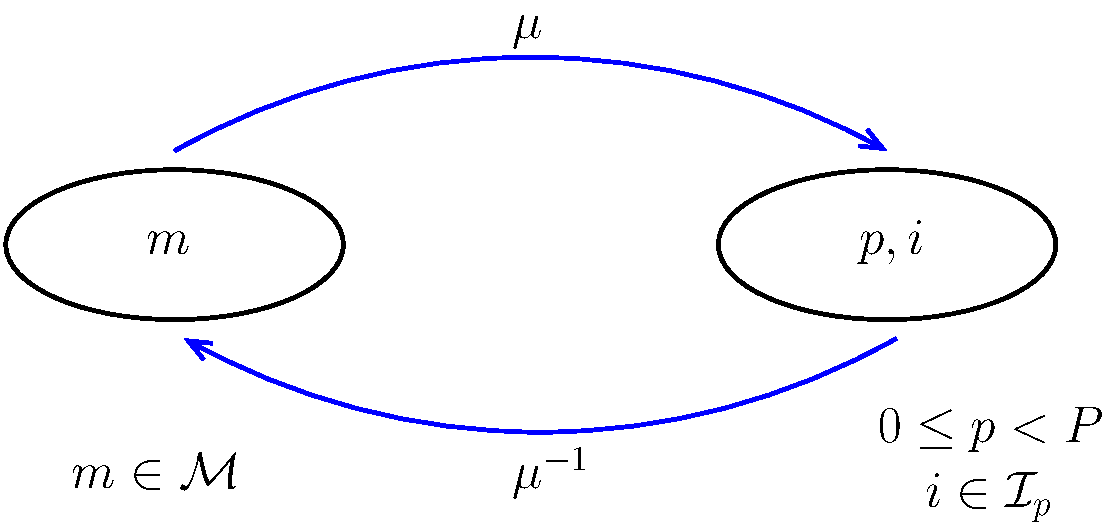
\includegraphics[width=10cm]{GlobalLocalMapping}
\end{center}
\end{frame}

\begin{frame}\frametitle{The innerproduct: distribution of work and data }
\begin{center}
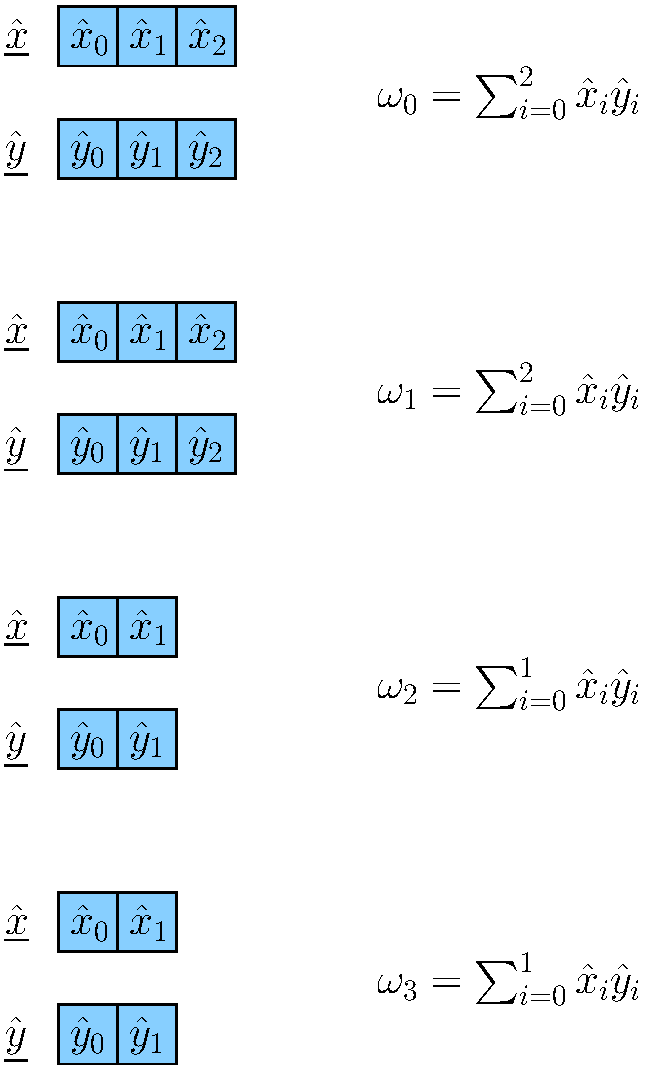
\includegraphics[width=4cm]{Vector3}
\end{center}
\end{frame}


\begin{frame}\frametitle{Improved sample "program" on processor $p$, ($0 \leq p < P$)}
\fbox{
  \addtolength{\linewidth}{-2\fboxsep}
  \addtolength{\linewidth}{-2\fboxrule}
  \begin{minipage}{\linewidth}
    $\hat x,\hat y:$ vectors of dimension $I_p$ (contiguous memory).

    \begin{align*}
      \omega_p &= \sum_{i=0}^{I_p-1} \hat x_i \, \hat y_i 
      = \sum_{i=0}^{I_p-1} x_{\mu^{-1}(p,i)}\,\, y_{\mu^{-1}(p,i)} 
      = \sum_{m \in \mathcal{M}_p} x_m \,y_m \\ \\
    &\text{Send } \omega_p \text{ to processor } q \not= p.\\
    &\text{Receive } \omega_q \text{ from processor } q \not= p.\\ \\
      \sigma &= \sum_{q=0}^{P-1} \omega_p.
    \end{align*}
  \end{minipage}
} 
\end{frame}

\begin{frame}\frametitle{Global reduction algorithms}
Reduction algorithm for 
\begin{align*}
\sigma = \sum_{p=0}^{P-1} \omega_p \qquad   \text{(global sum)}
\end{align*}

%The corresponding MPI-calls are:\\
\begin{align*}
  &\text{\textcolor{red}{MPI\_Reduce}}(\sigma,\omega,1,\text{MPI\_REAL},\text{MPI\_SUM},0,\text{MPI\_COMM\_WORLD}) \\
  &\text{{\em (the answer will end up on processor $0$)}} \\
  \intertext{or}
  &\text{\textcolor{red}{MPI\_Allreduce}}(\sigma,\omega,1,\text{MPI\_REAL},\text{MPI\_SUM},\text{MPI\_COMM\_WORLD} ) \\
  &\text{{\em (the answer will be known to every processor)}}
\end{align*}
\end{frame}

\begin{frame}\frametitle{Global sum ($P=4$)}
\begin{center}
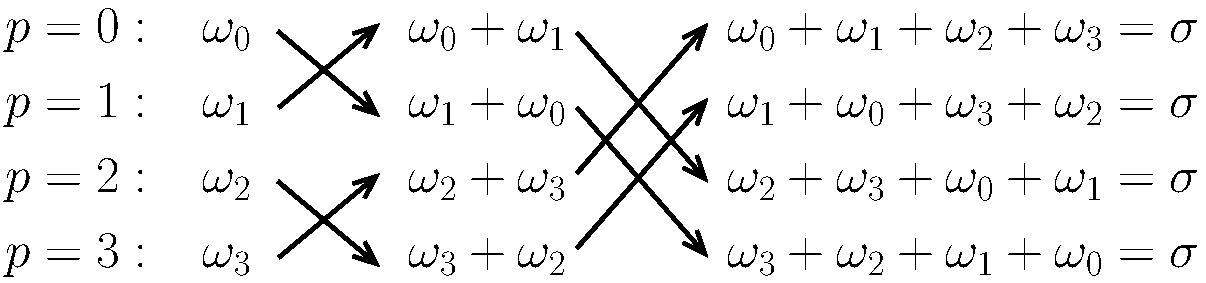
\includegraphics[width=10cm]{Allreduce}
\end{center}
\vspace{1cm}
Can be completed in $\log_2(P)$ steps  \\
\vspace{1cm}
\textcolor{red}{MPI\_Allreduce} 
\end{frame}

\begin{frame}\frametitle{Final "program" on processor $p$, ($0 \leq p < P$)}
\fbox{
  \addtolength{\linewidth}{-2\fboxsep}
  \addtolength{\linewidth}{-2\fboxrule}
  \begin{minipage}{\linewidth}
    $\hat x,\hat y:$ vectors of dimension $I_p$.

    \begin{equation*}
      \omega_p = \sum_{i=0}^{I_p-1} \hat x_i \,\hat y_i = \sum_{i=0}^{I_p-1} x_{\mu^{-1}(p,i)} \,\, y_{\mu^{-1}(p,i)} = \sum_{m \in \mathcal{M}_p} x_m \,y_m
    \end{equation*}
    
    \begin{align*}
      \text{Set } \sigma&=\omega_p \\
      \text{for } d&=0,\ldots,D-1 \quad (D = \log_2 P) \\
      &\text{Send } \sigma \text{ to processor } q = p \bar{\vee} 2^d \\
      &\text{Receive } \sigma_q \text{ from processor } q = p \bar{\vee} 2^d \\
      &\sigma=\sigma+\sigma_q \\
      \text{end } &
    \end{align*}
    where $\bar{\vee}$ is exclusive OR\\ ($q = p \bar{\vee} 2^d$ means that processor
    $q$ differs from processor $p$ only in bit $d$).  \\
  \end{minipage}
 } 
\end{frame}

\end{document}
